\setcounter{chapter}{1} % previous chapter number

\chapter{Special functions}
\label{h:special}

\begin{quote}
We must admit with humility that, while number is purely a product of our minds, space has a reality outside our minds, so that we cannot completely prescribe its properties a priori.

-- Carl Friedrich Gauss, letter to Bessel
\end{quote}

\begin{quote}
We are servants rather than masters in mathematics.

--- Charles Hermite
\end{quote}

%\setcounter{page}{1} 
\minitoc

In this chapter, we will solve the wave equations for a few special geometries. Firstly for the case of a medium with cylindrical symmetry, which will allow us to introduce Bessel, Neumann and Hankel functions. Secondly, we will look at higher order solutions of the paraxial wave equation, which requires the use of Hermite polynomials.

\section{Bessel functions}

\subsection{Bessel's differential equation}\label{sec-bessel-eq}

In the previous chapter, we derived the Helmholtz equation Eq.~\ref{eq-helmholtz}. Writing this in cylindrical coordinates gives

\begin{equation}
\frac{\partial^2 \psi}{\partial r^2} + \frac{1}{r} \frac{\partial \psi}{\partial r} +\frac{1}{r^2} \frac{\partial^2 \psi}{\partial \theta^2} + \frac{\partial^2 \psi}{\partial z^2} + k_0^2 n^2\psi = 0 \label{eq-helmholtz-cyl}
\end{equation}

Here, $\psi$ can represent any of the Cartesian components of the electric or magnetic field, or the axial coordinates $E_z$ and $H_z$ in cylindrical coordinates.

We assume that we are looking at a region of space where $n$ is constant. Let's try a solution of the following form, with $k_\theta$ and $k_z$ constant: 

\begin{equation}
\psi(r,\theta,z) = R(r)e^{-j k_\theta \theta }e^{-j k_z z} \\
\end{equation}  

Later in this chapter, we will deal with the physical interpretation behind this expression. For the time being, let's just substitute it in the Helmholtz equation. This leads to

\begin{equation}
\frac{d^2 R(r)}{d r^2} + \frac{1}{r} \frac{d R(r)}{d r} + \left[k_0^2 n^2 - k_z^2 - \frac{k_\theta^2}{r^2} \right] R(r) = 0
\end{equation} 

Or

\begin{equation}
r^2\frac{d^2 R(r)}{d r^2} + r \frac{d R(r)}{d r} + \left[ r^2 (k_0^2 n^2 - k_z^2)- k_\theta^2 \right] R(r) = 0
\end{equation}

We make the following change of variables:

\begin{equation}
x = r \sqrt{k_0^2 n^2 - k_z^2} \stackrel{def}{=} k_t r
\end{equation}

Renaming $R$ to $X$ and $k_\theta$ to $\nu$ we get

\begin{equation}
\fbox{$\displaystyle
x^2\frac{d^2 X(x)}{d x^2} + x \frac{d X(x)}{d x} + \left(x ^ 2 - \nu^2 \right)X(x) = 0 \label{eq-bessel}
$}
\end{equation}

Eq.~\ref{eq-bessel} is called Bessel's differential equation. A solution to this equation is given by $J_\nu(x)$, the Bessel function of the first kind of order $\nu$.

In what follows, we will mostly consider the important special case where $\nu$ is an integer. In this situation, we will use the notation $J_n(x)$, where $n$ is the integer version of $\nu$ and is not to be confused with the refractive index $n$ in Eq.~\ref{eq-helmholtz-cyl}.

\subsection{Generating function for integer order}

To investigate the properties of Bessel functions, it is instructive to define them through a \emph{generating function}. Let's introduce a function of two variables:

\begin{equation}
g(x,t) \stackrel{def}{=} e^{x/2(t-1/t)} \label{eq-gen-bessel}
\end{equation}

When we expand this function in a Laurent series in $t$, we \emph{define} the coefficients as being the Bessel functions:

\begin{equation}
e^{x/2(t-1/t)}  \stackrel{def}{=} \sum_{n = - \infty}^{\infty} J_n(x)t^n \label{eq-g-bessel}
\end{equation}  

Later, we will show that the functions $J_n(x)$ defined in this way do indeed satisfy Bessel's differential equation Eq.~\ref{eq-bessel}. For now, let's start with deriving a series expansion for $J_n(x)$ by expanding the exponentials in Eq.~\ref{eq-g-bessel}:

\begin{equation}
e^{xt/2} \cdot e^{-x/2t} = \sum_{r = 0}^{\infty} {\left(\frac{x}{2}\right)}^r \frac{t^r}{r!} \cdot \sum_{s = 0}^{\infty} {(-1)}^s { \left(\frac{x}{2}\right)}^s \frac{t^{-s}}{s!}
\end{equation} 

Introducing a new variable $n = r - s$ and getting rid of $r$, we can reorganise this equation to give

\begin{equation}
e^{xt/2} \cdot e^{-x/2t} = \sum_{n = -\infty}^{\infty} \left[ \sum_{s = 0}^{\infty} {\left(\frac{x}{2}\right)}^{n+s} \frac{1}{(n+s)!} \cdot (-1)^s {\left(\frac{x}{2}\right)}^{s} \frac{1}{s!} \right] t^n
\end{equation} 

This means that

\begin{equation}
\fbox{$\displaystyle
J_n(x) = \sum_{s = 0}^{\infty} \frac {{(-1)}^s}{s!(n+s)!} {\left(\frac{x}{2}\right)}^{n+2s} \label{eq-bessel-series}
$}
\end{equation} 

This series expansion can be used to numerically calculate the Bessel functions. Fig.~\ref{fig-bessel-J} plots $J_0(x)$, $J_1(x)$, $J_2(x)$. These functions oscillate, but are not periodic.

\begin{figure}
\centering
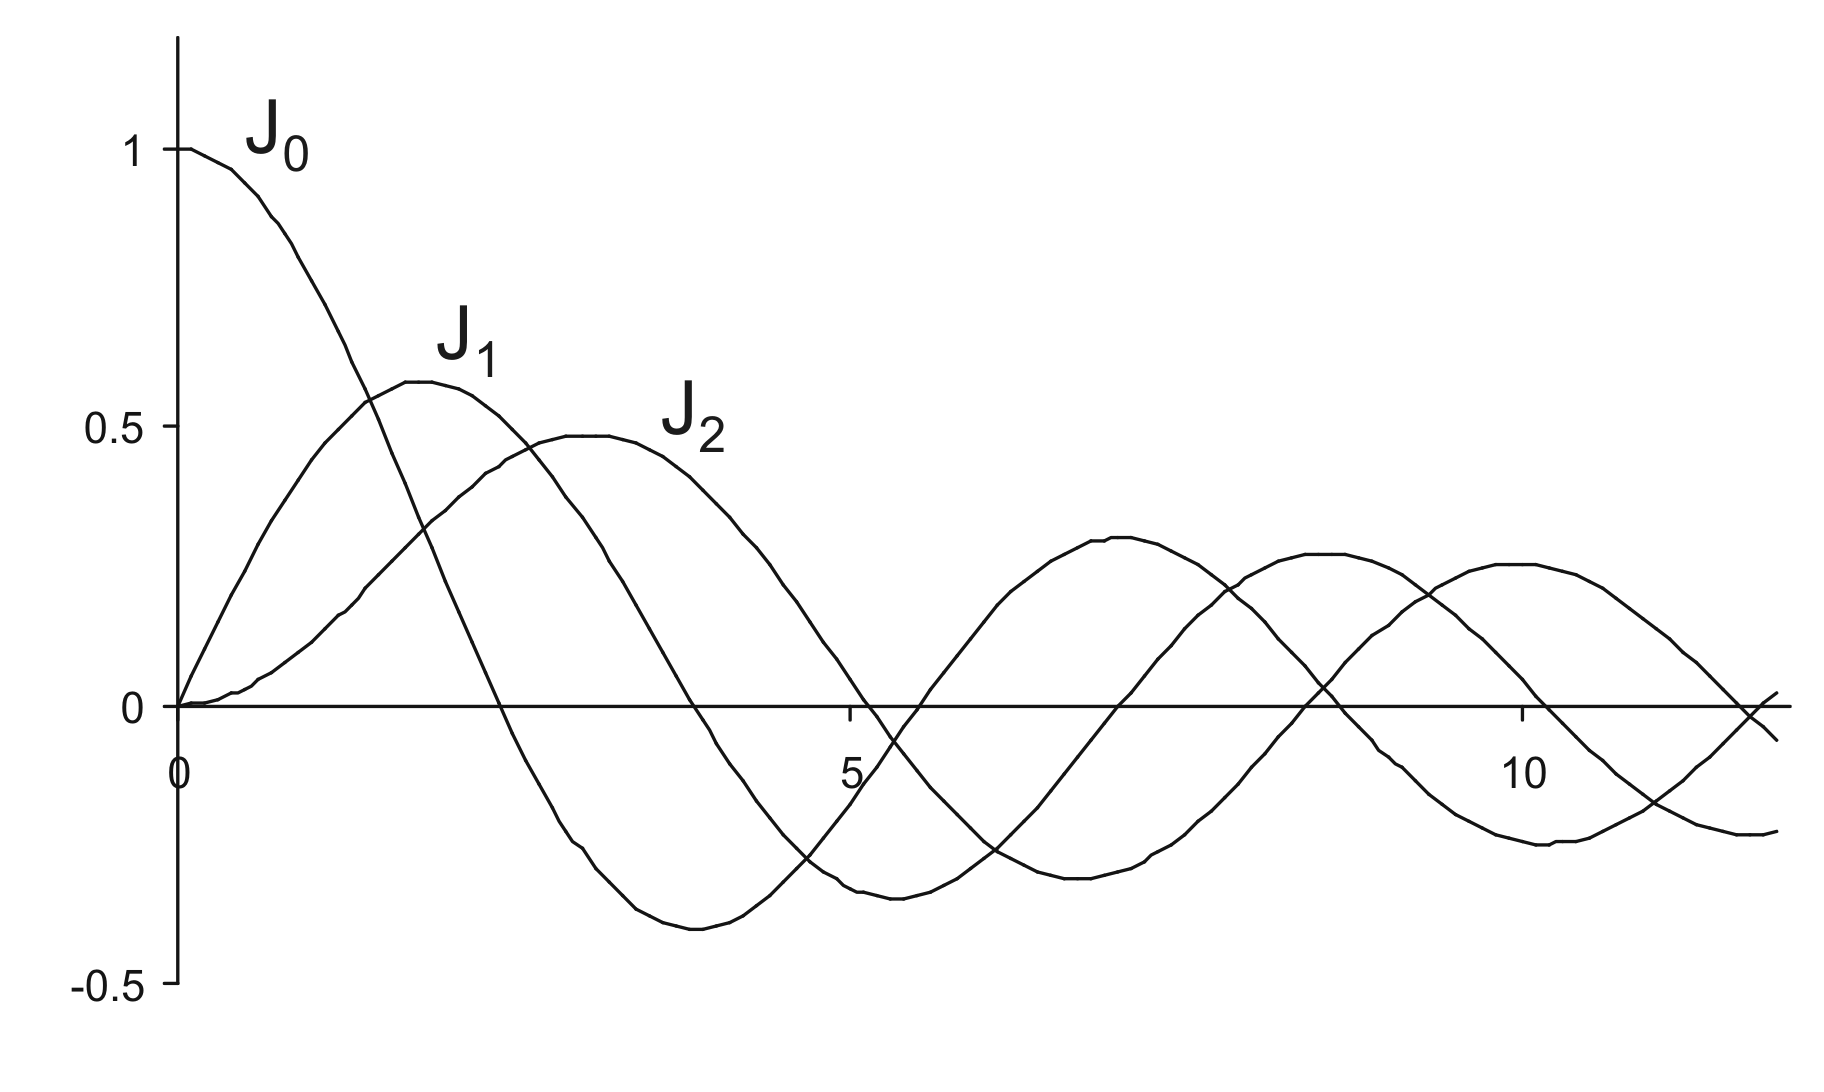
\includegraphics[scale=0.7]{special/figures/j}
\caption{The Bessel functions $J_0(x)$, $J_1(x)$ and $J_2(x)$.}
\label{fig-bessel-J}
\end{figure}

\begin{sidebar}
\begin{ex}
Show that
$$\lim_{x \to 0} \frac{J_1(x)}{x}= \frac{1}{2}$$
\end{ex}
\end{sidebar}

\begin{sidebar}
\begin{ex}
Use the definition of the generating function Eq.~\ref{eq-g-bessel} to show that
$$J_{-n}(x)=(-1)^nJ _n(x)$$
Hint: try replacing $t$ by $-1/t$ in the generating function.
\end{ex}
\end{sidebar}

\begin{sidebar}
\begin{ex}
Use the product of the generating functions $g(x,t)$ and $g(x,-t)$ to show that
$$\left[ J_0(x) \right]^2 + 2 \sum_{n=1}^\infty \left[ J_n(x) \right]^2 = 1 $$
\end{ex}
\end{sidebar}

\begin{sidebar}
\begin{ex}
By evaluating the generation function in a suitable point, prove the following
$$ \cos x =  J_0(x) + 2 \sum_{n=1}^\infty (-1)^n J_{2n}(x)  $$
$$ \sin x =  2 \sum_{n=0}^\infty (-1)^n J_{2n+1}(x)  $$
\end{ex}
\end{sidebar}

\begin{sidebar}
\begin{ex}
Evaluate the following contour integral along the unit circle in the complex $t$-plane:

$$ \oint_C t^{-n-1} g(x,t) dt $$

In doing so, derive the following equations:

$$J_n(x) = \frac {1}{2\pi} \int_0 ^ {2 \pi} \cos (n \theta - x \sin \theta ) d\theta $$

$$ J_0(x) =  \frac {1}{2\pi} \int_0 ^ {2 \pi}  e^{j x \cos \theta} d \theta $$
\end{ex}
\end{sidebar}


\subsection{Recurrence relations}

If we differentiate Eq.~\ref{eq-g-bessel} with respect to $t$, we get

\begin{equation}
\frac{x}{2}\left({1 + \frac{1}{t^2}}\right) e^{x/2(t-1/t)} = \sum_{n = - \infty}^{\infty} n J_n(x)t^{n-1}
\end{equation}

Substituting Eq.~\ref{eq-g-bessel} back into this, we get


\begin{equation}
\frac{x}{2}\left({1 + \frac{1}{t^2}}\right) \sum_{n = - \infty}^{\infty} J_n(x)t^n = \sum_{n = - \infty}^{\infty} n J_n(x)t^{n-1}
\end{equation} 

Equating the coefficients of like powers of $t$ we get

\begin{equation}
\frac{x}{2} J_n(x) + \frac{x}{2} J_{n+2}(x) = (n+1)J_{n+1}(x)
\end{equation} 

Or with the substitution $n+1 \to n$

\begin{equation}
\fbox{$\displaystyle
J_{n-1}(x) + J_{n+1}(x) = \frac{2n}{x} J_n(x)
$}
\end{equation} 

\begin{sidebar}
\begin{ex}
Differentiate the generating function with respect to $x$ to show that
$$\fbox{$\displaystyle J_{n-1}(x) - J_{n+1}(x) = 2 J_n'(x)$}$$ \label{ex-recur}
\end{ex}
\end{sidebar}

\begin{sidebar}
\begin{ex}
Show that
$$\begin{array}{lcll}a) & J_{n-1}(x) = \frac{n}{x}J_n(x) + J_n'(x) \\b) & J_{n+1}(x) = \frac{n}{x}J_n(x) - J_n'(x) \\c) & \frac{d}{dx}\left[x^n J_n(x)\right] = x^n J_{n-1}(x) \\d) & \frac{d}{dx}\left[x^{-n} J_n(x)\right] = -x^{-n} J_{n+1}(x)\end{array}$$ \label{ex-recurrence}
\end{ex}
\end{sidebar}


\begin{sidebar}
\begin{ex}
First, show that
$$\int_0^\infty J_1( x) dx =  1$$
Then, extend this to show that
$$\int_0^\infty J_1( x) dx = \int_0^\infty J_3( x) dx = \int_0^\infty J_5( x) dx = \cdots = 1$$
\end{ex}
\end{sidebar}

\begin{sidebar}
\begin{ex}
Show that
$$\int_0^1 x^3 J_0(k x) dx =  \frac{J_1(k)}{k} - 2 \frac{J_2(k)}{k^2}$$
If $k$ is a zero of $J_0$, show that this integral is equal to
$$\frac{J_1(k)}{k^3}\left(k^2-4\right)$$
\end{ex}
\end{sidebar}

\begin{sidebar}
\begin{ex}
Fraunhofer diffraction is governed by the following equation (see the course \emph{Microphotonics}):

$$U(x_0, y_0) \sim \iint_{-\infty}^{\infty} U(x_1, y_1) e ^{j \frac{2\pi}{\lambda z} (x_0 x_1 + y_0 y_1)} dx_1 dy_1  $$

By using polar coordinates both in the aperture plane

$$x_1 = \rho_1 \cos \theta_1; \quad y_1 = \rho_1 \sin \theta_1$$

and the observation plane

$$x_0 = \rho_0 \cos \theta_0; \quad y_0 = \rho_0 \sin \theta_0$$

show that for rotationally symmetric apertures this reduces to

$$U(\rho_0) \sim  \int_0^{\infty} \int_0^{2 \pi} U(\rho_1)  e ^{j \frac{2\pi}{\lambda z} \rho_0 \rho_1 \cos \theta_1} \rho_1 d\rho_1 d\theta_1  $$

Then, proceed to calculate the so-called Airy diffraction pattern for a circular aperture of radius $a$:

$$U(\rho_0) \sim \frac {J_1\left( 2 \pi \frac {\rho_0 a}{\lambda z} \right)}{\frac{\rho_0}{\lambda z a}}$$

\end{ex}
\end{sidebar}

\subsection{Bessel's differential equation revisited}

From Ex. \ref{ex-recurrence}, we get

\begin{equation}
J_{n-1}(x) = \frac{n}{x}J_n(x) + J_n'(x)
\end{equation}

This can be written as

\begin{equation}
x J_n'(x) + n J_n(x) - x J_{n-1}(x) = 0 \label{eq-bessel-dif-rec}
\end{equation} 

Differentiating with respect to $x$, we get

\begin{equation}
J_n'(x) + x J_n''(x) + n J_n'(x) - J_{n-1}(x) - x J_{n-1}'(x)= 0
\end{equation} 

or after multiplying by $x$:

\begin{equation}
x^2 J_n''(x) + (n + 1) x J_n'(x) - x J_{n-1}(x) - x^2 J_{n-1}'(x)= 0
\end{equation} 

We now subtract Eq.~\ref{eq-bessel-dif-rec} multiplied by $n$:

\begin{equation}
x^2 J_n''(x) + (n + 1) x J_n'(x) - x J_{n-1}(x) - x^2 J_{n-1}'(x) - n\left(x J_n'(x) + n J_n(x) - x J_{n-1}(x)\right)= 0
\end{equation} 

This simplifies to

\begin{equation}
x^2 J_n''(x) +  x J_n'(x) - x^2 J_{n-1}'(x) - n^2 J_n(x) + (n - 1) x J_{n-1}(x)= 0 \label{eq-bessel-dif-rec-2}
\end{equation} 

As a next step, we now take another recurrence equation from Ex. \ref{ex-recurrence}:

\begin{equation}
J_{n+1}(x) = \frac{n}{x}J_n(x) - J_n'(x)
\end{equation} 

Replacing $n$ with $n-1$, this can be written as

\begin{equation}
x J_{n}(x) = (n-1)J_{n-1}(x) - x J_{n-1}'(x)
\end{equation} 

With this, we can eliminate $J_{n-1}$ and $J_{n-1}'$ from Eq.~\ref{eq-bessel-dif-rec-2}:

\begin{equation}
x^2 J_n''(x) +  x J_n'(x) + x^2 J_n(x) - n^2 J_n(x) = 0
\end{equation} 

This is nothing other than Bessel's differential equation Eq.~\ref{eq-bessel}.

This shows that any function satisfying the recurrence relations used (also for non--integer values of $n$), also satisfies Bessel's equation. This is true in particular for the functions defined through our generating function Eq.~\ref{eq-gen-bessel}.

\subsection{Fourier--Bessel series}

Bessel functions can be used as a basis set for a series expansion of an arbitrary function. Before we can tackle this, we require some orthogonality relations for which we need to calculate a certain type of integral.

\subsubsection{Lommel's integral}

Consider the following two differential equations:

\begin{equation}
x^2 \frac{d^2 \phi}{dx^2}  + x \frac{d \phi}{dx} + \left(l^2x^2 - n^2\right) \phi = 0 \label{eq-bessel-orth-1}
\end{equation} 

\begin{equation}
x^2 \frac{d^2 \psi}{dx^2}  + x \frac{d \psi}{dx} + \left(k^2x^2 - n^2\right) \psi = 0 \label{eq-bessel-orth-2}
\end{equation} 

Solutions to these equations are $J_n(lx)$ and $J_n(kx)$ respectively. By multiplying Eq.~\ref{eq-bessel-orth-1} with $\psi/x$, Eq.~\ref{eq-bessel-orth-2} with $\phi/x$ and subtracting the two results, we get

\begin{equation}
x \left( \frac{d^2 \phi}{dx^2}\psi - \frac{d^2 \psi}{dx^2} \phi \right) + \left(\psi \frac{d \phi}{dx}- \frac{d \psi}{dx}\phi\right) + \left(l^2 - k^2\right) x \phi \psi = 0
\end{equation}

This can be written as

\begin{equation}
\frac{d}{dx}\left[x \left( \frac{d \phi}{dx} \psi - \frac{d \psi}{dx} \phi\right)\right] = \left(k^2 - l^2\right) x \phi \psi
\end{equation}

such that

\begin{equation}
x \left[{\frac{dJ_n(lx)}{dx}  J_n(kx) - \frac{dJ_n(kx)}{dx} J_n(lx)}\right] + C = \left(k^2 - l^2\right)\int x J_n(lx)J_n(kx)dx
\end{equation}

With prime denoting derivation with respect to the \emph{entire} argument, we have $dJ_n(kx)/dx = kJ_n'(kx)$ and $dJ_n(lx)/dx = lJ_n'(lx)$, such that for $l \ne \pm k$

\begin{equation}
\int x J_n(lx)J_n(kx)dx = \frac{x}{k^2 - l^2} \left[{l J_n'(lx) J_n(kx) -  k J_n'(kx) J_n(lx)}\right] + C \label{eq-lommel-1}
\end{equation} 

The second recurrence relation from Ex. \ref{ex-recurrence} takes the form

\begin{equation}
J_n'(lx) =  \frac{n}{lx}J_n(lx)-J_{n+1}(lx)
\end{equation} 

Likewise,
\begin{equation}
J_n'(kx) =  \frac{n}{kx}J_n(kx)-J_{n+1}(kx)
\end{equation} 

So, Eq.~\ref{eq-lommel-1} becomes

\begin{equation}
\int x J_n(lx)J_n(kx)dx = \frac{x}{k^2 - l^2} \left[{k J_{n+1}(kx) J_n(lx) - l J_{n+1}(lx) J_n(kx)}\right] + C \label{eq-lommel-2}
\end{equation} 

Eq.~\ref{eq-lommel-2} is called Lommel's integral.

\subsubsection{Orthogonality}

Suppose that $\xi_i$ and $\xi_j$ are two different zeros of $J_n(x)$. Then, from Lommel's integral Eq.~\ref{eq-lommel-2}, it immediately follows that

\begin{equation}
\fbox{$\displaystyle
\int_0^1 x J_n(\xi_i x)J_n(\xi_j x)dx = 0 \label{eq-bessel-ortho}
$}
\end{equation} 

This can be seen as an orthogonality condition that $J_n(\xi_i x)$ and $J_n(\xi_j x)$ satisfy.

\subsubsection{Fourier--Bessel series}

Eq.~\ref{eq-bessel-ortho} can be used to expand functions in a so--called \emph{Fourier--Bessel} series. Suppose $\xi_i$ is the set of zeros of $J_n(x)$. (One can prove that all $\xi_i$ are real and that there is an infinite number of them.) For a function $f(x)$ defined in the interval $[0,1]$, we can write:

\begin{equation}
f(x) = \sum_{i=0}^{\infty} a_i J_n(\xi_i x) \label{eq-fourier-bessel}
\end{equation} 

To determine the unknown coefficients $a_i$, we multiply Eq.~\ref{eq-fourier-bessel} by $x J_n(\xi_m x)$ and integrate over $[0,1]$. Thanks to the orthogonality relations, we get

\begin{equation}
\int_0^1 x J_n(\xi_m x) f(x) dx = a_m \int_0^1 x J_n^2(\xi_m x) dx \label{eq-fourier-bessel-2}
\end{equation} 

The integral on the left--hand side of Eq.~\ref{eq-fourier-bessel-2} can be calculated analytically or numerically, depending on the nature of $f(x)$. To evaluate the integral on the right--hand side of \ref{eq-fourier-bessel-2}, we cannot use Lommel's integral Eq.~\ref{eq-lommel-2}, because $k=l$. So we need to calculate this normalisation integral in a different way, which we will do now.

\subsubsection{Normalisation}

We need to calculate

\begin{equation}
I = \int x J_n^2(k x) dx
\end{equation}

which after a change of variables $kx = t$ becomes

\begin{equation}
I = \frac{1}{k^2} \int t J_n^2(t) dt
\end{equation}

Partial integration yields

\begin{equation}
I = \frac{t^2}{2 k^2}J_n^2(t) - \frac{1}{k^2} \int t^2 J_n(t) J_n'(t) dt
\end{equation} 

But $J_n(t)$ is a solution of Bessel's equation Eq.~\ref{eq-bessel}, such that

\begin{equation} 
- t^2 J_n(t) = t^2 J_n''(t) + t J_n'(t) - n^2 J_n(t)
\end{equation}

Multiplying this by $J_n'(t)$ we get

\begin{align} 
- t^2 J_n(t) J_n'(t) = & t^2 J_n''(t)J_n'(t) + t J_n'^2(t) - n^2 J_n(t)J_n'(t) \nonumber \\
 = & \frac{1}{2} \left[{t^2 J_n'^2(t) - n^2 J_n^2(t)}\right]'
\end{align}

So finally

\begin{equation}
I = \frac{t^2}{2 k^2}J_n^2(t) + \frac{1}{2 k^2} \left[{t^2 J_n'^2(t) - n^2 J_n^2(t)}\right] + C
\end{equation} 

or

\begin{equation}
\int x J_n^2(k x) dx = \frac{x^2}{2}\left[{J_n'^2(kx) + \left(1 - \frac{n^2}{k^2x^2}\right) J_n^2(kx)}\right] + C
\end{equation} 

Returning to our normalisation integral in Eq.~\ref{eq-fourier-bessel-2}, we get that

\begin{equation}
\int_0^1 x J_n^2(\xi_m x) dx = \frac{1}{2}\left[{J_n'^2(\xi_m) + \left(1 - \frac{n^2}{\xi_m^2}\right) J_n^2(\xi_m)}\right] + \frac{n^2}{2\xi_m^2} J_n^2(0)
\end{equation} 

This reduces to

\begin{align}
\int_0^1 x J_n^2(\xi_m x) dx =& \frac{1}{2}J_n'^2(\xi_m) + \frac{n^2}{2\xi_m^2} J_n^2(0) \nonumber \\
 =& \frac{1}{2}J_{n+1}^2(\xi_m) + \frac{n^2}{2\xi_m^2} J_n^2(0) \nonumber \\
 =& \frac{1}{2}J_{n+1}^2(\xi_m)
\end{align} 

where the second step makes use of the recurrence relations and the fact that $\xi_m$ is a zero of $J_n(x)$. The last transition is based on the fact that $J_n(0)=0$ for $n \ne 0$ (see Fig.~\ref{fig-bessel-J} or Eq.~\ref{eq-bessel-series}).

So, finally we get from Eq.~\ref{eq-fourier-bessel-2} the following expression for the expansion coefficients in the Fourier--Bessel series:

\begin{equation}
\fbox{$\displaystyle
a_m = \frac{2}{J_{n+1}^2(\xi_m)}\int_0^1 x J_n(\xi_m x) f(x) dx
$}
\end{equation} 

\begin{sidebar}
\begin{ex}
Show that
$$-\frac{1}{2} \ln x = \sum_{i=0}^{\infty} \frac{J_0(\xi_i x)}{\xi_i^2 J_1^2(\xi_i)}$$
where $\xi_i$ are the zeros of $J_0(x)$.
\end{ex}
\end{sidebar}

\subsection{Neumann and Hankel functions}

From the theory of differential equations, it can be derived that Bessel's equation has two linearly independent solutions. One of them is the Bessel function of the first kind $J_\nu(x)$. It can be shown that a second independent solution is given by the Bessel function of the second kind defined by

\begin{equation}
\fbox{$\displaystyle
Y_\nu(x) = \frac{\cos(\nu \pi)J_\nu(x) - J_{-\nu}(x)}{\sin(\nu \pi)}
$}
\end{equation} 

This function is sometimes also called the \emph{Neumann} or the Weber function, and sometimes symbolised by $N_\nu(x)$.

Fig.~\ref{fig-bessel-Y} plots the Neumann functions of the lowest three orders. Note the logarithmic type singularity at $x=0$.

\begin{figure}
\centering
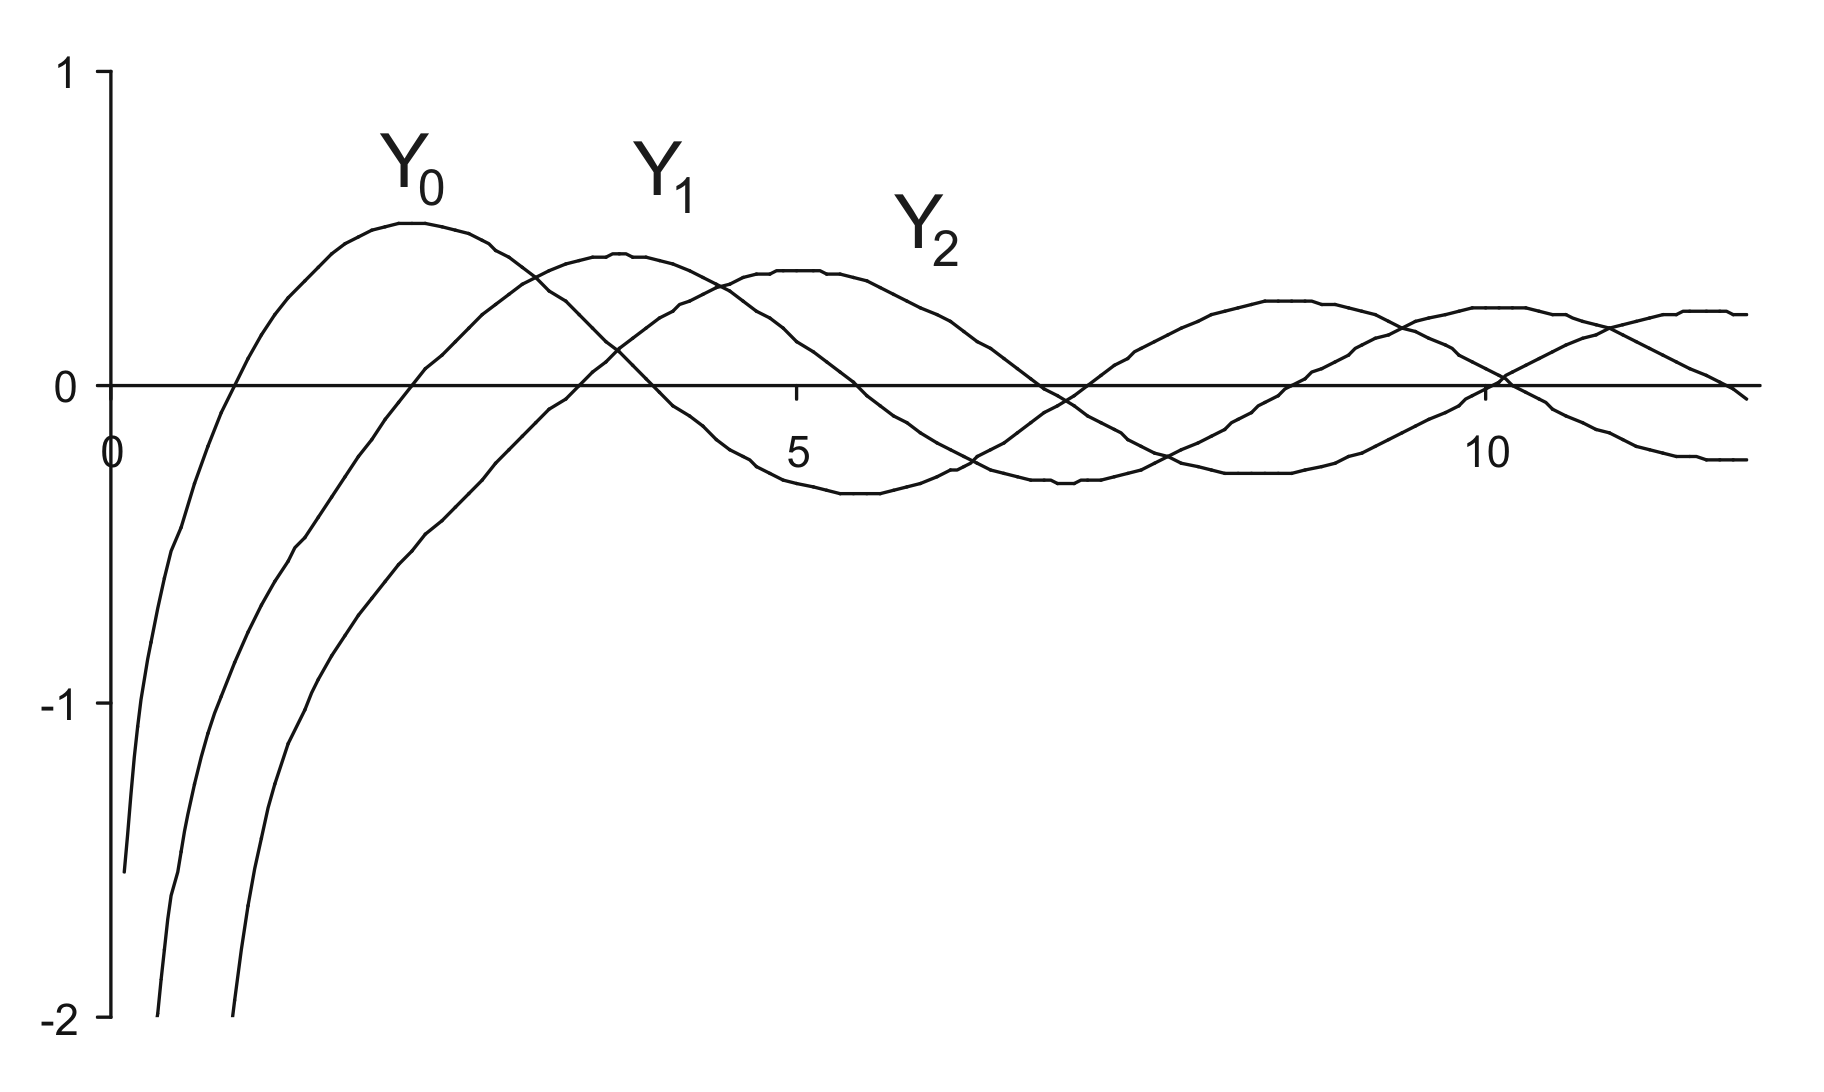
\includegraphics[scale=0.7]{special/figures/y}
\caption{The Neumann functions $Y_0(x)$, $Y_1(x)$ and $Y_2(x)$.}
\label{fig-bessel-Y}
\end{figure}

So the general solution of Bessel's equation can be written as

\begin{equation}
f(x) = A J_{\nu}(x) + B Y_{\nu}(x)
\end{equation} 

Of course, any other linearly independent combination of $J_{\nu}(x)$ and $Y_{\nu}(x)$ can also be used to express the solution, e.g.

\begin{equation}
f(x) = C H_{\nu}^{(1)}(x) + D H_{\nu}^{(2)}(x)
\end{equation} 

Here, $H_{\nu}^{(1)}(x)$ and $H_{\nu}^{(2)}(x)$ are the \emph{Hankel} functions of the first and second kind respectively, defined by

\begin{subequations}
\begin{equation}
\fbox{$\displaystyle H_{\nu}^{(1)}(x) = J_{\nu}(x) + j Y_{\nu}(x)$}
\end{equation} 
\begin{equation}
\fbox{$\displaystyle H_{\nu}^{(2)}(x) = J_{\nu}(x) - j Y_{\nu}(x)$}
\end{equation} 
\label{eq-hankel}
\end{subequations} 

Of course, if we are solving Eq.~\ref{eq-helmholtz-cyl} instead of Eq.~\ref{eq-bessel}, the arguments of the functions above are $k_t r$ instead of $x$. It is instructive to compare these functions to the solutions of the Helmholtz equation in a 1D Cartesian coordinate system:

\begin{equation}
f''(x) + k^2 f(x) = 0 \label{eq-helmholtz-1D}
\end{equation} 

The solutions of Eq.~\ref{eq-helmholtz-1D} are

\begin{equation}
f(x) = A \cos(kx) + B \sin(kx)
\end{equation} 

The sine and cosine solutions are oscillating solutions which can be interpreted physically as standing waves. Note the correspondence to $J_n(x)$ and $Y_n(x)$ which are also oscillating functions. Therefore, they can be thought of as the representation of standing waves in a circular coordinate system, with the only difference that $Y_n(x)$ diverges at the origin.

Another way of writing the solutions of Eq.~\ref{eq-helmholtz-1D} is

\begin{equation}
f(x) = C e^{jkx} + D e^{-jkx}
\end{equation} 

because $e^{\pm j \theta} = \cos \theta \pm j \sin \theta$ (compare this to Eq.~\ref{eq-hankel}).

Physically, $e^{-jkx}$ corresponds to an outgoing wave travelling towards $x=+\infty$, while $e^{jkx}$ is an incoming wave from $x=+\infty$ \footnote{This is for a choice of $e^{j \omega t}$ as time dependence in the definition of phasors. Some authors choose $e^{-j \omega t}$ as time dependence, and then $e^{-jkx}$ is an incoming wave.}.

It can be proven that for large $x$ the following asymptotic expansions hold:
$H_{\nu}^{(1)}(x) \sim e^{jx}$ and  $H_{\nu}^{(2)}(x) \sim e^{-jx}$. So, $H_{\nu}^{(2)}(x)$ is the cylindrical equivalent of an outgoing plane wave, while $H_{\nu}^{(1)}(x)$ is an incoming plane wave.

Whether to use Bessel/Neumann functions or rather Hankel functions to represent the solution of Bessel's differential equation, is usually determined by physical and/or practical considerations, as we will illustrate next for the case of finding eigenmodes in an optical fibre.

\subsection{Application: the eigenmodes of an optical fibre}

Consider the optical fibre from Fig.~\ref{fig-fibre}: a central core with radius $R$ made of a material with refractive index $n_1$, surrounded by a cladding with refractive index $n_2 < n_1$. The cladding is taken to be infinitely thick. 

\begin{figure}
\centering
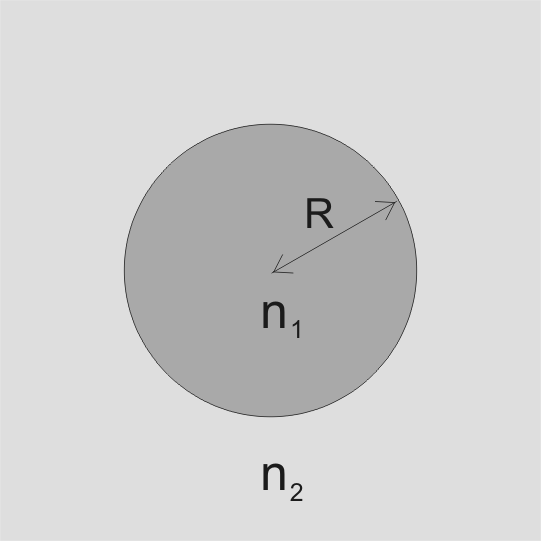
\includegraphics{special/figures/fibre}
\caption{Optical fibre.}
\label{fig-fibre}
\end{figure}

Fields in the optical fibre have to satisfy the Helmholtz equation. Just like in Section~\ref{sec-bessel-eq}, we propose solutions of the form 

\begin{equation}
\psi(r,\theta,z) = R(r)e^{-j k_\theta \theta }e^{-j k_z z} \\
\end{equation}  

These kinds of solutions are actually the eigenmodes of this particular waveguide, because of the form of their $z$--dependence\footnote{These eigenmodes propagate along $z$. Contrast this with the treatment of bent waveguides in the previous chapter, where the $z$--dimension didn't come in play because of the 2D nature of the problem and where the propagation was essentially along $\theta$.}.  Also, the fields must be periodic in the $\theta$--direction with period $2 \pi$. This means $k_\theta$ has to be an integer, which we will call $l = 0, \pm 1, \pm 2, \ldots$.

As we've seen before, $R$ has to satisfy this equation:

\begin{equation}
r^2\frac{d^2 R(r)}{d r^2} + r \frac{d R(r)}{d r} + \left[{r^2 \left(k_0^2 n^2(r) - k_z^2\right) - l^2}\right]R(r) = 0 \label{eq-fibre-0}
\end{equation} 

We define $k_{t,i}^2=k_0^2 n_i^2 - k_z^2$, where $i=1$ for the core and $i=2$ for the cladding.

We already know that in each of the regions $i$ the solutions of Eq.~\ref{eq-fibre-0} are Bessel functions of order $l$ with argument $k_{t,i} r$.

For the core, we write the general solution as

\begin{equation}
R(r) = A J_l\left(k_{t,1}r\right) + B Y_l\left(k_{t,1}r\right), \hspace{0.5 cm} r<R \label{eq-fibre-1}
\end{equation} 

But since the Neumann functions diverge at $r=0$, it immediately follows that $B=0$.

For the cladding, it is more advantageous to write the general solution in terms of Hankel functions:

\begin{equation}
R(r) = C H_l^{(1)}\left(k_{t,2}r\right) + D H_l^{(2)}\left(k_{t,2}r\right), \hspace{0.5 cm} r>R \label{eq-fibre-2}
\end{equation} 

For physical reasons, there can only be outgoing waves towards infinity, so $C=0$. Note that contrary to $k_{t,1}$, $k_{t,2}$ is imaginary for $k_0 n_2 < k_z < k_0 n_1$, so the fields for guided modes are exponentially decaying in the cladding.

So far, the treatment has been fully vectorial because solutions of the form (\ref{eq-fibre-1}) and (\ref{eq-fibre-2}) have to written both for $E_z$ and $H_z$, and these two fields couple because of the continuity conditions at $r=R$. For the sake of simplicity, we will only consider a scalar approximation here, where the modes are approximately TEM and the continuity conditions are simplified to the continuity of $R$ and $d R / d r$. This approximation turns out to be valid for weakly guided fibres where $n_1 \approx n_2$.

Imposing the continuity of $R$ and $d R / dr$ leads to

\begin{equation}
A J_l\left(k_{t,1}R\right) = D H_l^{(2)}\left(k_{t,2}R\right)
\end{equation} 

\begin{equation}
A k_{t,1} J'_l\left(k_{t,1}R\right) = D k_{t,2} H_l'^{(2)}\left(k_{t,2}R\right)
\end{equation} 

This only has non--trivial solutions if

\begin{equation}
\frac{J_l\left(k_{t,1}R\right)}{k_{t,1} J'_l\left(k_{t,1}R\right)} = \frac{H_l^{(2)}\left(k_{t,2}R\right)}{k_{t,2} H_l'^{(2)}\left(k_{t,2}R\right)} \label{eq-disp-fibre}
\end{equation}

Since $k_{t,1}$ and $k_{t,2}$ are functions of $k_z$, Eq.~\ref{eq-disp-fibre} can be used to calculate the $k_z$'s of the eigenmodes of the fibre. After that, the field profiles can be calculated from Eq.~\ref{eq-fibre-1} and \ref{eq-fibre-2}.

\begin{sidebar}
\begin{ex}
Solve the Helmholtz equation in free space in cylindrical coordinates. Look at the evolution of the intensity of the solution as a function of $z$. What do you notice? These modes are called \emph{Bessel beams}.
\end{ex}
\end{sidebar}

\section{Hermite polynomials}

In the Bachelor's level Photonics course, Gaussian beams were introduced as solutions to the paraxial wave equation. We will briefly review this material, and then go on to look for higher--order solutions to this equation. In this process, Hermite polynomials will pop up and we will study their properties as a model for other orthogonal polynomials.

\subsection{The paraxial wave equation and Gaussian beams}

The paraxial wave equation is an approximation to the Helmholtz equation under the so--called slowly varying envelope approximation (SVEA). This approximation looks for solutions which are essentially plane waves propagating along the $z$--direction, but which are modulated by a slowly varying function $A({\bf r})$:

\begin{equation}
\psi({\bf r}) = A({\bf r})e^{-jkz}
\end{equation} 

So,

\begin{equation}
\frac{\partial \psi({\bf r})}{\partial z} = \frac {\partial A({\bf r})}{\partial z}e^{-jkz} -j k A({\bf r})e^{-jkz}
\end{equation} 

and

\begin{equation}
\frac{\partial^2 \psi({\bf r})}{\partial z^2} = \frac{\partial^2 A({\bf r})}{\partial z^2}e^{-jkz} - 2 j k \frac{\partial A({\bf r})}{\partial z}e^{-jkz} - k^2 A({\bf r})e^{-jkz}
\end{equation} 

The fact that $A({\bf r})$ is a slowly varying function of $z$ means that we can neglect $\partial^2 A / \partial z^2$ with respect to $j k \partial A / \partial z$in the previous equation. With this, the Helmholtz equation reduces to

\begin{equation}
\fbox{$\displaystyle
\nabla_T^2 A({\bf r}) -2jk \frac{\partial A({\bf r})}{\partial z} = 0
$}
\label{eq-paraxial}
\end{equation} 

Here, $\nabla_T^2$ stands for the transverse part $(\partial^2 / \partial x^2) + (\partial^2 / \partial y^2)$ of the Laplacian operator.

A solution to this equation is the Gaussian beam, which is given by

\begin{equation}
A_G({\bf r}) = \frac{1}{q(z)}e^{-\frac{jk\rho^2}{2q(z)}} \label{eq-gauss}
\end{equation}   

where $q(z)=z+jb_0$. 

In this context, the function $W(z)$ is defined as

\begin{equation}
W(z)=\sqrt{\frac{2 b_0}{k} \left(1 + \frac{z^2}{b_0^2}\right)} \label{eq-W}
\end{equation} 

$W(z)$ can be interpreted as the beam width of the Gaussian beam.

\subsection{Higher--order solutions of the paraxial wave equation}

Let's try to find a modulated version of the Gaussian beam which also satisfies the paraxial wave equation:

\begin{equation}
A(x,y,z) = X\left({\frac{\sqrt{2}x}{W(z)}}\right) Y\left({\frac{\sqrt{2}y}{W(z)}}\right) e^{-jZ(z)} A_G(x,y,z) \label{eq-gauss-higher}
\end{equation} 

Here, $A_G$ is the Gaussian beam from Eq.~\ref{eq-gauss} and $X()$, $Y()$ and $Z()$ are three real--valued functions that we still need to determine such that Eq.~\ref{eq-gauss-higher} satisfies the paraxial Helmholtz equation.

For the derivatives of Eq.~\ref{eq-gauss-higher} we get

\begin{equation}
\frac{\partial A}{\partial x} = \frac{\sqrt{2}}{W}X'Ye^{-jZ} A_G + XYe^{-jZ} \frac{\partial A_G}{\partial x} 
\end{equation} 

and

\begin{equation}
\frac{\partial^2 A}{\partial x^2} = \frac{2}{W^2}X''Ye^{-jZ} A_G  + 2\frac{\sqrt{2}}{W}X'Ye^{-jZ} \frac{\partial A_G}{\partial x}  + XYe^{-jZ} \frac{\partial^2 A_G}{\partial x^2}
\end{equation} 

Or, using Eq.~\ref{eq-gauss} to calculate $\partial A_G / \partial x$:

\begin{equation}
\frac{\partial^2 A}{\partial x^2} = \frac{2}{W^2}X''Ye^{-jZ} A_G  - 2j k x \frac{\sqrt{2}}{qW}X'Ye^{-jZ}A_G  + XYe^{-jZ} \frac{\partial^2 A_G}{\partial x^2} \label{eq-hermite-gauss-1}
\end{equation} 

and similar equations for the $y$--derivatives. For the $z$--derivative we get

\begin{align}
\frac{\partial A}{\partial z} =  -\frac{\sqrt{2}x W'}{W^2}X'Ye^{-jZ} A_G -\frac{\sqrt{2}y W'}{W^2}XY'e^{-jZ} A_G \nonumber \\ 
+ XY\left(-jZ'\right)e^{-jZ} A_G + XYe^{-jZ}\frac{\partial A_G}{\partial z} \label{eq-hermite-gauss-2}
\end{align} 

Let's substitute this in the paraxial equation Eq.~\ref{eq-paraxial}. Because $A_G$ is itself a solution of this equation, the last terms from Eq.~\ref{eq-hermite-gauss-1} and \ref{eq-hermite-gauss-2} cancel and we get:

\begin{align}
\frac{2}{W^2}\left(X''Y+XY''\right)e^{-jZ} A_G   \nonumber \\
-2jk \frac{\sqrt{2}}{Wq}\left(xX'Y+yXY'\right)e^{-jZ}A_G \nonumber \\
+2jk \frac{\sqrt{2} W'}{W^2}\left(xX'Y+yXY'\right)e^{-jZ}A_G \nonumber \\
-2jk XY\left(-jZ'\right)e^{-jZ} A_G = 0
\end{align}

Getting rid of the common factors and dividing by $XY$, we get

\begin{equation}
\frac{1}{W^2}\left(\frac{X''}{X}+\frac{Y''}{Y}\right)  
- j k \left(\frac{\sqrt{2}}{Wq} - \frac{\sqrt{2}W'}{W^2}\right)\left(x\frac{X'}{X}+y\frac{Y'}{Y}\right)
-kZ' = 0
\end{equation} 

or
\begin{equation}
\left(\frac{X''}{X}+\frac{Y''}{Y}\right)  
- j k  \left(\frac{W^2}{q} - W'W\right)\frac{\sqrt{2}}{W}\left(x\frac{X'}{X}+y\frac{Y'}{Y}\right)
-kW^2Z' = 0
\end{equation} 

Using the definitions for $W$ and $q$, it follows that $W^2/q - W'W = -j \lambda / \pi$. If we now perform the change of variables $u = \sqrt(2) x / W(z)$ and  $v = \sqrt(2) y / W(z)$, we get

\begin{equation}
\left[{\frac{X''(u)}{X(u)} - 2 u\frac{X'(u)}{X(u)}}\right] + 
\left[{\frac{Y''(v)}{Y(v)} - 2 v\frac{Y'(v)}{Y(v)}}\right] -kW^2(z)Z'(z) = 0
\end{equation} 

The left--hand side of this equation is a sum a three terms, each of which is a function of a single independent variable ($u$, $v$ and $z$ respectively). Therefore, each of these terms must be equal to a constant. Equating the first term to $-2\mu_1$ and the second to $-2\mu_2$, the third must be equal to $2(\mu_1+\mu_2)$. This separation of variables leads to the following ordinary differential equations:

\begin{equation}
X''(u) - 2 u X'(u) = - 2 \mu_1 X(u) \label{eq-diff-hermite-0}
\end{equation} 

\begin{equation}
Y''(v) - 2 v Y'(v) = - 2 \mu_2 Y(v)
\end{equation} 

\begin{equation}
b_0\left(1 + \frac{z^2}{b_0^2}\right)Z'(z) = -(\mu_1+\mu_2)
\end{equation} 

From this, it follows immediately that $Z(z) = -(\mu_1+\mu_2) \arctan(z/b_0)$. However, the differential equations for $X$ and $Y$ have no obvious solutions at first sight. In the next sections, we will show that their solutions are \emph{Hermite polynomials}, and that $\mu_1$ and $\mu_2$ are integers.

In similar vein to the treatment of Bessel functions, we will start by introducing a generating function and then continue to derive recurrence relations which will lead to a differential equation.

\subsection{Generating function fo the Hermite polynomials}

The generating function of the Hermite polynomials takes the following form:

\begin{equation}
g(x,t) = e^{-t^2 + 2tx} \label{eq-gen-hermite}
\end{equation}

The Hermite polynomials $H_n(x)$ are \emph{defined} from the the Laurent series in $t$ of $g(x,t)$ as 

\begin{equation}
e^{-t^2 + 2tx}= \sum_{n = 0}^{\infty} H_n(x)\frac{t^n}{n!} \label{eq-g-hermite}
\end{equation} 

Note the absence of a superscript in $H_n(x)$, which distinguishes them from the unrelated Hankel functions.

\begin{sidebar}
\begin{ex}
Show that
$$H_n(x) = \sum_{r=0}^{\lfloor n/2 \rfloor}(-1)^r {(2x)}^{n-2r} \frac{n!}{(n-2r)! r!}$$
\end{ex}
\end{sidebar}

\subsection{Recurrence relations for Hermite polynomials}

Similar to the treatment of Bessel functions, we can derive recurrence relations by differentiating the generating function.

E.g. by differentiating Eq.~\ref{eq-g-hermite} with respect to $t$, we get

\begin{equation}
(-2t+2x)e^{-t^2 + 2tx} = \sum_{n = 0}^{\infty} H_n(x) \frac{nt^{n-1}}{n!}
\end{equation} 

Substituting Eq.~\ref{eq-g-hermite} back in this, we get

\begin{equation}
(-2t+2x) \sum_{n = 0}^{\infty} H_n(x)\frac{t^n}{n!} = \sum_{n = 0}^{\infty} H_n(x) \frac{nt^{n-1}}{n!}
\end{equation} 

This leads to

\begin{equation}
-2  \frac{H_{n-1}(x)}{(n-1)!} + 2 x \frac{H_n(x)}{n!} = H_{n+1}(x) \frac{n+1}{(n+1)!}
\end{equation} 

where $n \geq 1$, or

\begin{equation}
\fbox{$\displaystyle
H_{n+1}(x) = 2 x H_n(x) - 2 n H_{n-1}(x)
$} \label{eq-recur-hermite-1}
\end{equation} 

Direct expansion of the generating function yields that $H_0(x) = 1$ and that $H_1(x) = 2x$. With this and Eq.~\ref{eq-recur-hermite-1}, we can iteratively construct all the Hermite polynomials. For reference, Table \ref{tab-hermite} lists the first Hermite polynomials. Fig.~\ref{fig-hermite} plots the first three Hermite polynomials.

\begin{figure}
\centering
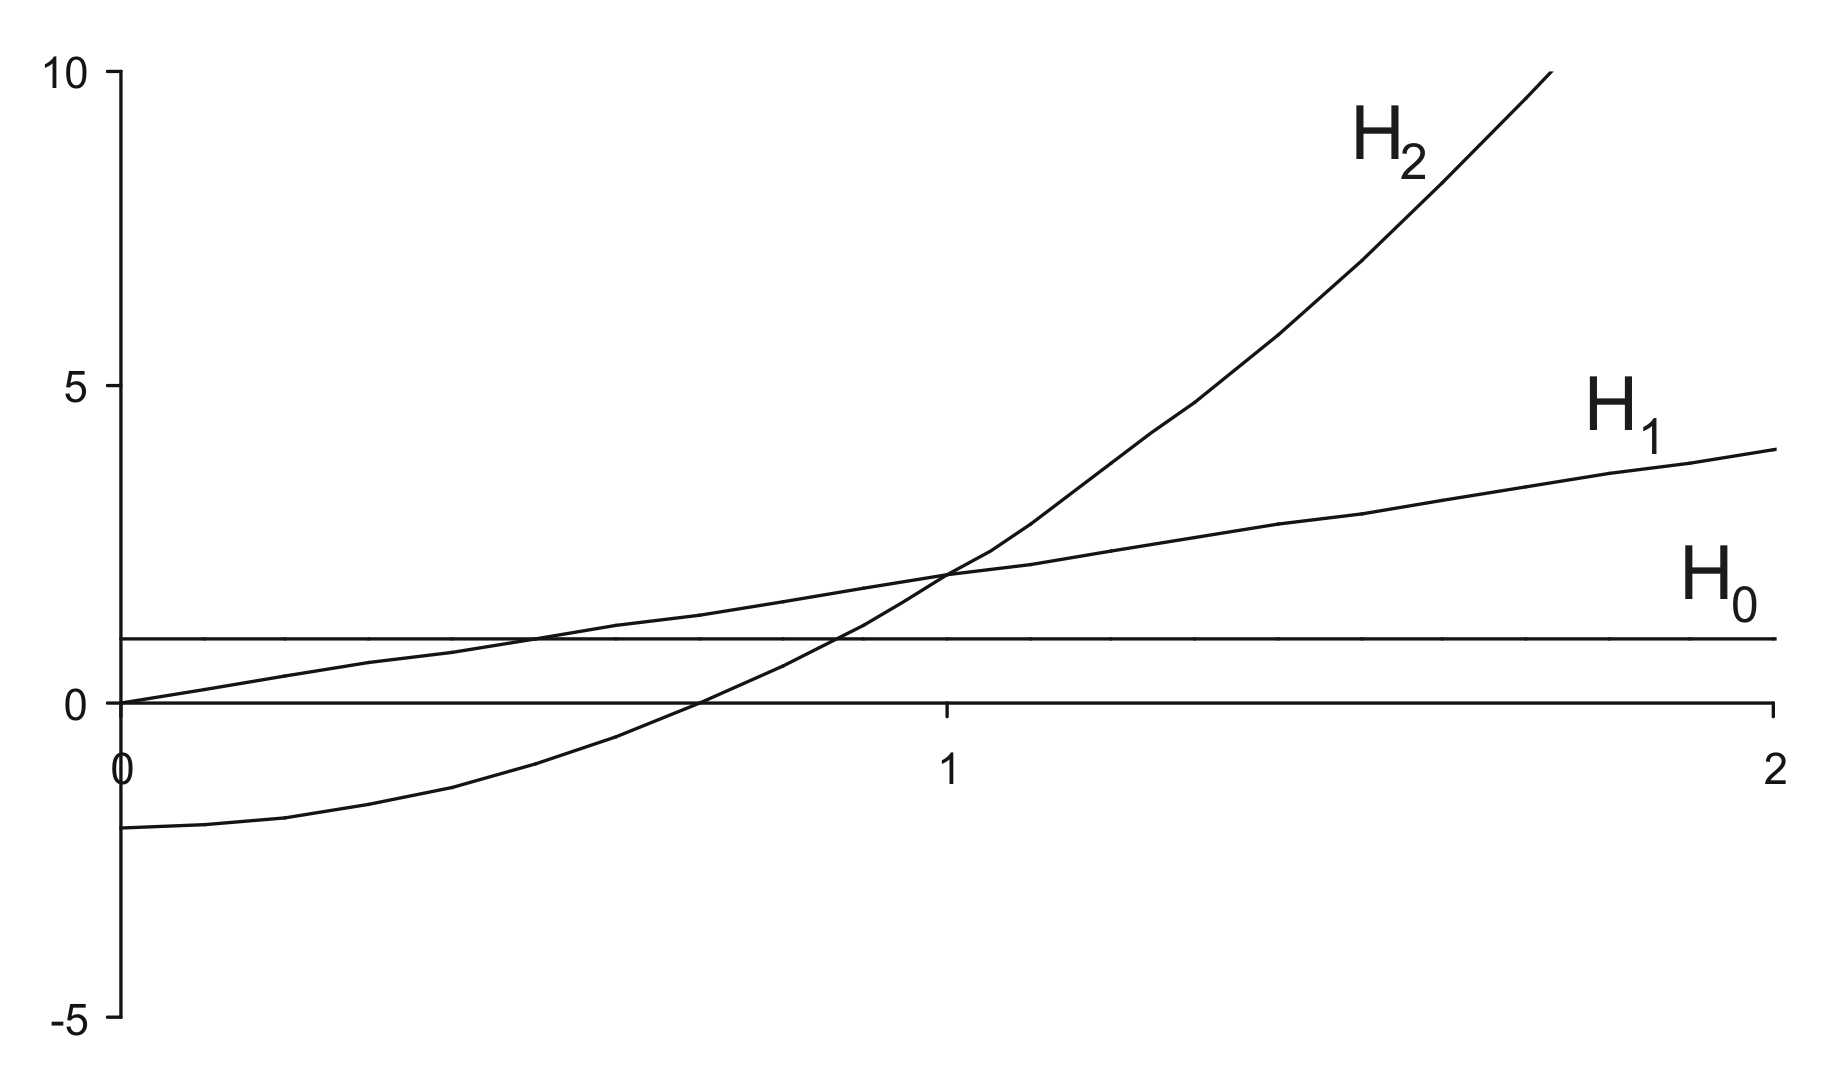
\includegraphics[scale=0.7]{special/figures/hermite}
\caption{The Hermite polynomials $H_0(x)$, $H_1(x)$, $H_2(x)$.}
\label{fig-hermite}
\end{figure}

\begin{table}
\begin{align}
H_0(x) = & 1 \nonumber \\
H_1(x) = & 2x \nonumber \\
H_2(x) = & 4x^2-2 \nonumber \\
H_3(x) = & 8x^3-12x \nonumber \\
H_4(x) = & 16x^4-48x^2+12 \nonumber \\
H_5(x) = & 32x^5-160x^3+120x \nonumber \\
H_6(x) = & 64x^6-480x^4+720x^2-120 \nonumber
\end{align}
\caption{Hermite polynomials}
\label{tab-hermite}
\end{table}  

\begin{sidebar}
\begin{ex}
Show that
$$\fbox{$\displaystyle H_n'(x) = 2nH_{n-1}(x)$}$$ \label{eq-recur-hermite-2}
\end{ex}
\end{sidebar}

\subsection{Hermite's differential equation}

Differentiating Eq.~\ref{eq-recur-hermite-1} with respect to $x$, we get

\begin{equation}
H_{n+1}'(x) = 2  H_n(x) + 2 x H_n'(x)- 2 n H_{n-1}'(x)
\end{equation} 

Using the results from  Ex. \ref{eq-recur-hermite-2}, we have $H_{n+1}'(x) = 2(n+1)H_n(x)$ and $2 n H_{n-1}'(x) = H_n''(x)$:

\begin{equation}
2(n+1)H_n(x) = 2  H_n(x) + 2 x H_n'(x)- H_n''(x)
\end{equation} 

This reduces to

\begin{equation}
\fbox{$\displaystyle
H_n''(x) - 2 x H_n'(x) + 2n H_n(x) = 0 \label{eq-diff-hermite-1}
$}
\end{equation} 

which is indeed Eq.~\ref{eq-diff-hermite-0}, with $\mu_1=n$.

Returning to our higher--order solutions of the paraxial wave equation, Fig.~\ref{fig-gauss-hermite} plots the field profile of some of these so--called \emph{Gauss--Hermite modes}. They are characterised by two integer indices, indicating the order of the Hermite polynomials for the $x$ and $y$ direction.

\begin{figure}
\centering
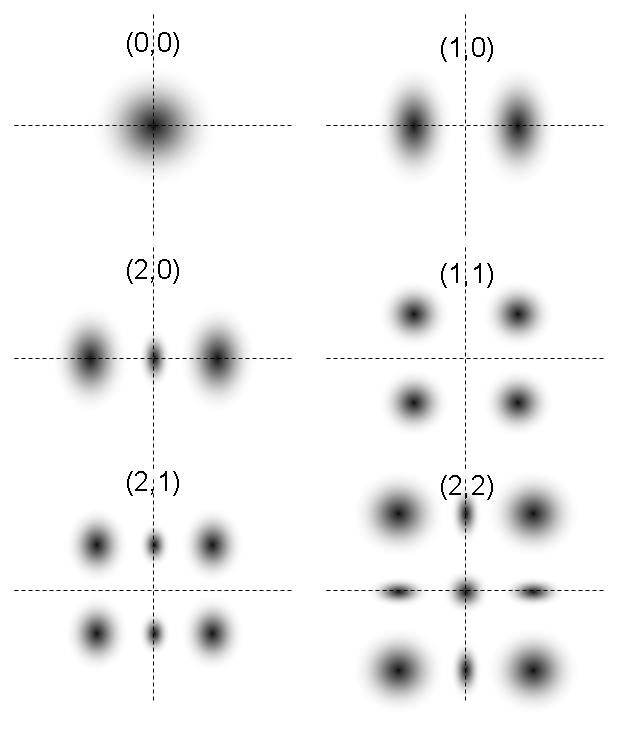
\includegraphics[scale=0.5]{special/figures/gauss}
\caption{Some Gauss--Hermite modes.}
\label{fig-gauss-hermite}
\end{figure}

\subsection{Orthogonality of Hermite polynomials}

Just as we did with Bessel functions, we can use Hermite polynomials to expand a function in a series. In order to do that, we will need to establish the correct orthogonality relation between Hermite polynomials and normalise them.

Consider the following two differential equations:

\begin{equation}
\phi'' - 2 x \phi' + 2m \phi = 0 \label{eq-hermite-ortho-1}
\end{equation}
\begin{equation}
\psi'' - 2 x \psi' + 2n \psi = 0 \label{eq-hermite-ortho-2}
\end{equation}

The solutions of these are $H_m(x)$ and $H_n(x)$ respectively. Multiplying Eq.~\ref{eq-hermite-ortho-1} by $\psi e^{-x^2}$, Eq.~\ref{eq-hermite-ortho-2} by $\phi e^{-x^2}$ and subtracting, we get

\begin{equation}
e^{-x^2}\left(\phi''\psi -\psi''\phi\right)- e^{-x^2} 2 x \left(\phi'\psi -\psi'\phi\right)+ e^{-x^2}2(m-n)\phi\psi = 0
\end{equation} 

This can be written as

\begin{equation}
\left[e^{-x^2}\left(\phi'\psi -\psi'\phi\right)\right]' = e^{-x^2}2(n-m)\phi\psi
\end{equation} 

Integrating this between $-\infty$ and $\infty$ we get

\begin{equation}
2(n-m)\int_{-\infty}^{\infty}e^{-x^2}\phi\psi dx = \left[e^{-x^2}\left(\phi'\psi -\psi'\phi\right)\right]_{-\infty}^{+\infty}
\end{equation} 

The right hand side is equal to zero, because $e^{-{\infty}^2}$ goes to zero more quickly than any polynomial.

So in the end we get

\begin{equation}
\fbox{$\displaystyle
\int_{-\infty}^{\infty}e^{-x^2}H_n(x)H_m(x)dx = 0, \hspace{0.5cm} n \ne m \label{eq-hermite-ortho}
$}
\end{equation} 

This is the orthogonality relation for Hermite polynomials: they are orthogonal over the interval $[-\infty, \infty]$ with the weighting function $e^{-x^2}$.

\subsection{Normalisation for Hermite polynomials}

To normalise the Hermite polynomials, we need to calculate

\begin{equation}
I = \int_{-\infty}^{\infty}e^{-x^2}H_n^2(x)dx
\end{equation}

We do this by multiplying the generating function Eq.~\ref{eq-g-hermite} by itself and by  $e^{-x^2}$:

\begin{equation}
e^{-x^2} e^{-t^2 + 2tx} e^{-s^2 + 2sx}= \sum_{m, n = 0}^{\infty}e^{-x^2} H_n(x)\frac{t^n}{n!}H_m(x)\frac{s^m}{m!}
\end{equation} 

When we integrate this over $x$ from $-\infty$ to $\infty$, the terms with $m \ne n$ on the right--hand side drop out because of the orthogonality relation Eq.~\ref{eq-hermite-ortho}:

\begin{equation}
\int_{-\infty}^{\infty} e^{-x^2} e^{-t^2 + 2tx} e^{-s^2 + 2sx} dx= \sum_{n = 0}^{\infty} \int_{-\infty}^{\infty} e^{-x^2} H_n^2(x)\frac{(st)^n}{n!n!} dx \label{eq-hermite-norm-1}
\end{equation} 

For the integral on the left--hand side, we get \footnote{To calculate $\int_{-\infty}^{\infty}e^{-x^2}dx$, write it as $\sqrt{\int_{-\infty}^{\infty} e^{-x^2}dx\int_{-\infty}^{\infty} e^{-y^2}dy}$ and transform it to polar coordinates with $x^2+y^2=r^2$ and $dxdy = r dr d\theta$.}

\begin{align}
\int_{-\infty}^{\infty} e^{-x^2} e^{-t^2 + 2tx} e^{-s^2 + 2sx} dx 
  = & \int_{-\infty}^{\infty} e^{-(x-s-t)^2} e^{2st}dx \nonumber \\
  = & \sqrt{\pi} e^{2st} \nonumber \\
  = & \sqrt{\pi} \sum_{n = 0}^{\infty} \frac{2^n{(st)}^n}{n!}  \label{eq-hermite-norm-2}
\end{align} 

By equating like powers of $st$ in the the right--hand sides of Eq.~\ref{eq-hermite-norm-1} and \ref{eq-hermite-norm-2} we get the value of the normalisation integral:

\begin{equation}
\int_{-\infty}^{\infty} e^{-x^2} H_n^2(x) dx = 2^n n! \sqrt{\pi}
\end{equation} 

With this we can finally write the complete expression to expand a function $f(x)$ in a series of Hermite polynomials:

\begin{equation}
f(x) = \sum_{n=0}^{\infty}a_n H_n(x)
\end{equation} 

with

\begin{equation}
\fbox{$\displaystyle
a_n = \frac{1}{2^n n!\sqrt{\pi}} \int_{-\infty}^{\infty} e^{-x^2} H_n(x) f(x) dx
$}
\end{equation} 

\subsection{Exercises}

\begin{sidebar}
\begin{ex}
Prove the following parity relation:
$$H_n(x) = (-1)^nH_n(-x)$$
a) by using the series expansion of Hermite polynomials
b) by replacing $t$ by $-t$ and $x$ by $-x$ in the generating function
\end{ex}
\end{sidebar}

\begin{sidebar}
\begin{ex}
Use the definition of the generating function for Hermite polynomials to prove that
$$H_{2n}(0) = (-1)^n \frac{(2n)!}{n!}$$
$$H_{2n+1}(0) = 0$$
\end{ex}
\end{sidebar}

\begin{sidebar}
\begin{ex}
Prove the Rodriguez formula for Hermite polynomials:
$$H_n(x) = (-1)^n e^{x^2}\frac{d^n}{d x^n}\left(e^{-x^2}\right)$$
\emph{Hint}: verify this formula for a few values of $n$ to get a feeling for how it works, and then use mathematical induction.
\end{ex}
\end{sidebar}

\begin{sidebar}
\begin{ex}
For $0 \leq m \leq n-1$, use the Rodriguez formula to show that 
$$\int_{-\infty}^{\infty}x^m e^{-x^2} H_n(x) dx = 0$$
\end{ex}
\end{sidebar}

\begin{sidebar}
\begin{ex}
Prove that 
$$ | H_n(x) | \le  | H_n(jx) | $$
\emph{Hint}: remove factors from the series expansion of $ H_n(jx) $ so that it contains only positive terms.
\end{ex}
\end{sidebar}


\begin{sidebar}
\begin{ex}
Show that 
$$\left( 2x - \frac{d}{dx} \right)^n 1 = H_n(x)$$
\emph{Hint}: verify this formula for a few values of $n$ to get a feeling for how it works, and then use mathematical induction.
\end{ex}
\end{sidebar}

\begin{sidebar}
\begin{ex}
Show that
$$ \int_{-\infty}^{\infty} e^{-x^2} x^2 H_n^2(x) dx = 2^{n-1} (2n + 1) n! \sqrt{\pi} $$
\emph{Hint}: expand $x H_n(x)$ using a recurrence relation and apply the orthogonality conditions.
This integral occurs in the calculation of the mean-square displacement of a quantum oscillator.
\end{ex}
\end{sidebar}

\begin{sidebar}
\begin{ex}
Expand the following integral in a power series in $t$

$$ \int_{-\infty}^{\infty} e^{-x^2/2} g(x,t) dx$$

and use the result to show that

$$\int_{-\infty}^{\infty} e^{-x^2/2} H_{2m}(x) dx = \frac{(2m)!}{m!} \sqrt{2\pi} $$
$$\int_{-\infty}^{\infty} e^{-x^2/2} H_{2m+1}(x) dx = 0 $$
\end{ex}
\end{sidebar}


\begin{sidebar}
\begin{ex}
Multiply the generating function by $t^{-k-1}$ and integrate over the unit circle in the complex $t$-plane to show that

$$H_k(x) =\frac{k!}{2 \pi j} \oint \frac{e^{-t^2 +2tx}}{t^{k+1}}dt $$

Then, show by direct substitution that this expression satisfies Hermite's differential equation. \emph{Hint}: try to write the integrand as a total differential.
\end{ex}
\end{sidebar}

\begin{sidebar}
\begin{ex}
Assume that based only on Hermite's differential equation, we managed to derive the recurrence relation involving $H_n'(x)$, as well as the values of $H_n(0)$. Based only on this information, derive the explicit form of the generating function $g(x,t)$ defined as

$$g(x,t) = \sum_{n = 0}^{\infty} H_n(x)\frac{t^n}{n!} $$

a) Take the derivative of $g(x,t)$ above with respect to $x$, use the recurrence relationship, and derive a first-order differential equation for $g(x,t)$.\\

b) Solve this equation to give

$$g(x,t) = e^{2tx} f(t)$$

c) Derive $f(t)$ by evaluating the expression for $x=0$.
\end{ex}
\end{sidebar}

\pagebreak
\section*{Friedrich Wilhelm Bessel (1784--1846)}

\parpic{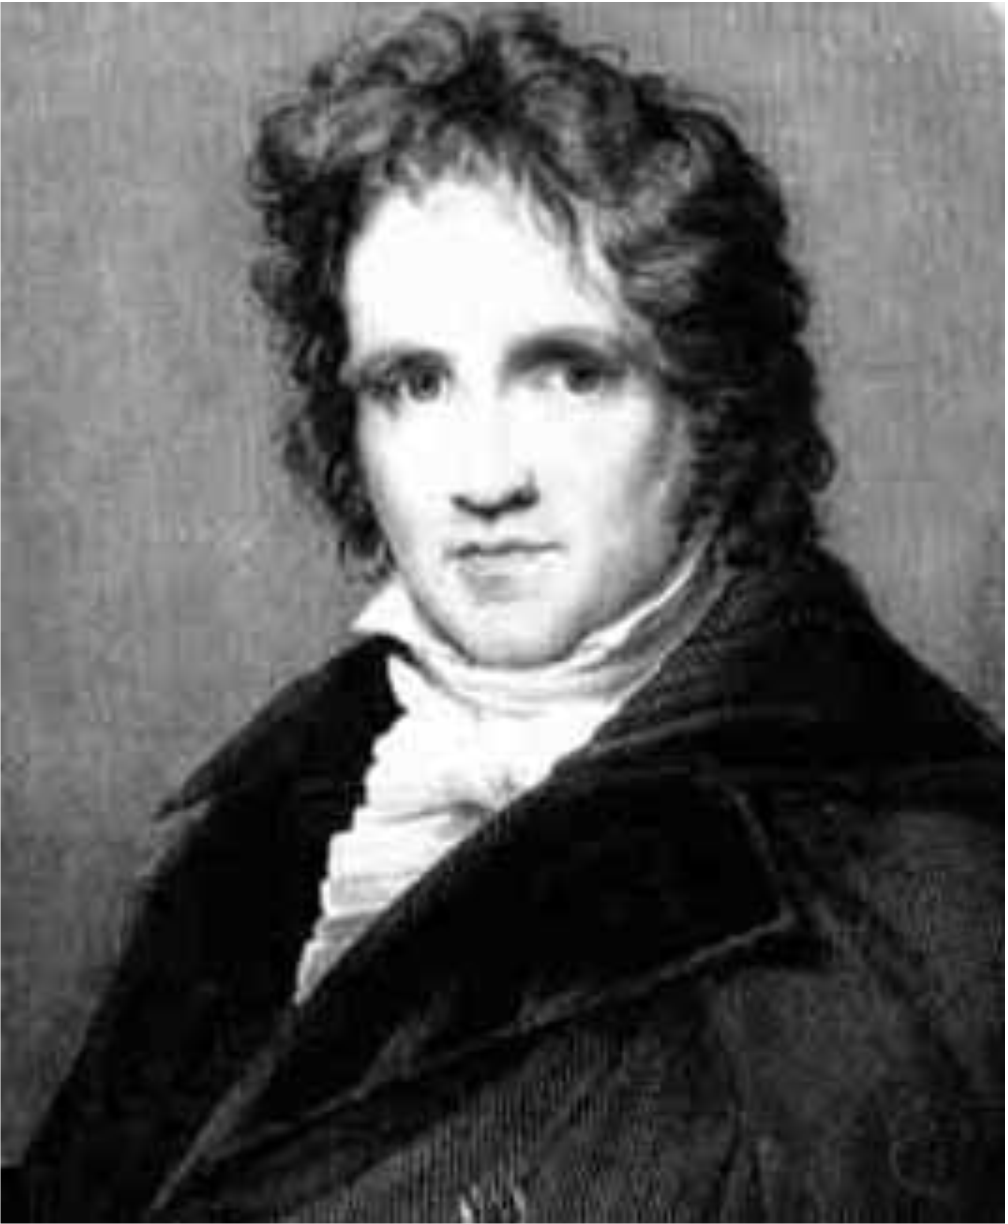
\includegraphics[scale=0.7]{special/figures/bessel}}

Friedrich Wilhelm Bessel was a German mathematician, astronomer, and systematiser of the Bessel functions (which, despite their name, were discovered by Daniel Bernoulli). He was born in Minden, Westphalia and died of cancer in K\"onigsberg (now Kaliningrad, Russia). He was a contemporary of Carl Gauss, also a mathematician and astronomer.
 
Bessel was the son of a civil servant, and at the age of 14 he was apprenticed to the import--export concern Kulenkamp. He shortly became an accountant for them, and the business' reliance on cargo ships led him to turn his mathematical skills to problems in navigation. This in turn led to an interest in astronomy as a way of determining longitude.
 
He came to the attention of a major figure of German astronomy at the time, Heinrich Wilhelm Olbers, by producing a refinement on the orbital calculations for Halley's Comet. Within two years he had left Kulenkamp and become an assistant at Lilienthal Observatory near Bremen, Germany. There he worked on James Bradley's stellar observations to produce precise positions for some 3222 stars.
 
 This work attracted considerable attention, and at the age of 26 he was appointed director of the K\"onigsberg Observatory by Frederick William III of Prussia. There he published tables of atmospheric refraction based on Bradley's observations, which won him the Lalande Prize from the Institut de France. On this base, he was able to pin down the position of over 50,000 stars during his time at K\"onigsberg.
 
 With this work under his belt, Bessel was able to achieve the feat for which he is best remembered today: he is credited with being the first to use parallax in calculating the distance to a star. Astronomers had believed for some time that parallax would provide the first accurate measurement of interstellar distances -- in fact, the 1830s housed a fierce competition between astronomers to be the first to accurately measure a stellar parallax. In 1838 Bessel won the "race", announcing that 61 Cygni had a parallax of 0.314 arcseconds; which, given the diameter of the Earth's orbit, indicated that the star was ~3 parsecs away. Hipparcos has calculated the parallax at 0.28547 arcseconds. He narrowly beat Friedrich Georg Wilhelm Struve and Thomas Henderson, who measured the parallaxes of Vega and Alpha Centauri in the same year.
 
 As well helping determine the parallax of 61 Cygni, Bessel's precise measurements allowed him to notice deviations in the motions of Sirius and Procyon, which he deduced must be caused by the gravitational attraction of unseen companions. His announcement of Sirius' "dark companion" in 1841 was the first correct claim of a previously unobserved companion by positional measurement, and eventually led to the discovery of Sirius B.
 
 Despite lacking a university education, Bessel was a major figure in astronomy during his lifetime. He was elected a fellow of the Royal Society, and the largest crater in the moon's Mare Serenitatis was named after him.


(from http://www.biographybase.com)